\documentclass{beamer}
\beamertemplatenavigationsymbolsempty
\usecolortheme{beaver}
\setbeamertemplate{blocks}[rounded=true, shadow=true]
\setbeamertemplate{footline}[page number]
%
\usepackage[utf8]{inputenc}
\usepackage[english,russian]{babel}
\usepackage{amssymb,amsfonts,amsmath,mathtext}
\usepackage{subfig}
\usepackage[all]{xy} % xy package for diagrams
\usepackage{array}
\usepackage{multicol}% many columns in slide
\usepackage{hyperref}% urls
\usepackage{hhline}%tables
% Your figures are here:
\graphicspath{ {fig/} {../fig/} }
\usepackage{float}

%----------------------------------------------------------------------------------------------------------
\title[\hbox to 56mm{Классификация по ОКПД2 }]{Классификация товаров \\ по ОКПД 2 кодам}
\author[С.\,А. Фирсов]{Сергей Андреевич Фирсов}
\institute{Московский физико-технический институт}
\date{\footnotesize
\par\smallskip\emph{Курс:} Автоматизация научных исследований\par (практика, В.\,В.~Стрижов)/Группа Б05-105
\par\smallskip\emph{Эксперт:} В.\,М.~Старожилец
\par\smallskip\emph{Консультант:} А.\,Е.~Вознюк
\par\bigskip\small 2024}
%----------------------------------------------------------------------------------------------------------
\begin{document}
%----------------------------------------------------------------------------------------------------------
\begin{frame}
\thispagestyle{empty}
\maketitle
\end{frame}
%-----------------------------------------------------------------------------------------------------


%----------------------------------------------------------------------------------------------------------
\begin{frame}{Постановка задачи}
Исследование направлено на решение задачи классификации товаров по кодам Общероссийского классификатора продукции по видам экономической деятельности (ОКПД 2) с использованием кратких текстовых описаний. \\
Выборка представлена парами "текстовое описание товара --- код ОКПД2".
$$\mathfrak{D}  = \{(\bold{x}_i, y_i)\}_{i=1}^{m},\; \bold{x}_i =  \{t_i\}_{j=1}^{n} \ \texttt{- т. описание},\; y_i \in \mathbf{Y}  = \{1, \dots, k\}.$$
Ограничения:
\begin{itemize}
  \item[\circ] Количество записей $m \approx 8$ миллионов, количество классов $k \approx 5000$. 
  \item[\circ] Структура классов несбалансирована: для некоторых классов доступно до 1000 записей, в то время как для других --- более 200000. 
  \item[\circ] Текстовые описания часто содержат узкоспециализированную лексику, жаргонизмы, артикулы и числовые значения, что усложняет задачу классификации.
\end{itemize}
\end{frame}

%----------------------------------------------------------------------------------------------------------
\begin{frame}{Определение модели}
Используется модель логистической регрессии
$$P(y=1 | \mathbf{x}; \boldsymbol{\theta_k}) = \sigma(\mathbf{x}^\top \boldsymbol{\theta_k}),$$
где $\mathbf{x}$ обозначает вектор признаков наблюдения (с предварительно добавленной единицей для учета свободного члена), $\boldsymbol{\theta_k}$ --- вектор параметров модели для класса $k$, а $\sigma(z) = \frac{1}{1 + e^{-z}}$ --- сигмоидная функция \\ 

\\ \bigskip \\
Функция потерь и задача оптимизации:
$$\mathcal{L}(\boldsymbol{\theta_k}) = -\frac{1}{N} \sum_{i=1}^{N} \left[ y_i \log(\sigma(\mathbf{x}_i^\top \boldsymbol{\theta_k})) + (1 - y_i) \log(1 - \sigma(\mathbf{x}_i^\top \boldsymbol{\theta_k})) \right],$$
$$\boldsymbol{\theta_k}^* = \arg\min_{\boldsymbol{\theta_k}} \mathcal{L}(\boldsymbol{\theta_k})$$
\end{frame}
%----------------------------------------------------------------------------------------------------------
\begin{frame}{Алгоритм решения}
Для преобразования текстов в векторное представление используются эмбеддинги, полученные с помощью библиотеки \texttt{spaCy}.\\
Для анализа текстовых данных и классификации используется модель логистической регрессии, реализованная в библиотеке \texttt{scikit-learn}.\\

Алгоритм решения:
\begin{enumerate}
    \item Предварительная обработка данных: очистка текста от шума, нормализация и токенизация.
    \item Фильтрация данных для улучшения свойств выборки.
    \item Преобразование текстов в векторное представление.
    \item Обучение модели логистической регрессии на обработанных данных.
    \item Оценка качества модели с roc-auc и pr-auc.
\end{enumerate}
\end{frame}

%----------------------------------------------------------------------------------------------------------
\begin{frame}{Описание данных и их предобработка}
Изначально данные --- это пары значений: текстовое описание товара и его ОКПД2 код. Эти описания были составлены людьми и могут содержать орфографические ошибки, лишние символы, артикли, цифры и многое другое.
\begin{itemize}
\item Данные очистили и типизировали.
\item В данных введено обозначение: префикс кода длины N (далее префикс N) --- первые N цифр кода.
\item Из-за вычислительной сложности эксперимента было принято выделить лишь несколько больших классов для анализа. 
\item Фильтрация для избавления от слишком мелких подклассов, чтобы избегать дизбаланса классов и улучшать качество классификации.
\end{itemize}
\end{frame}
%----------------------------------------------------------------------------------------------------------
\begin{frame}{Условия эксперимента}
\begin{itemize}
    \item Модель \texttt{"sklearn.linear\_model.LogisticRegression"}
    \item Предобученная модель NLP \texttt{"ru\_core\_news\_lg"}
     \item Проводились отдельные эксперименты с библиотекой \texttt{"gensim"}, для получения другой вариации эмбеддингов. Но результаты классификации оказались значительно хуже.
    \item Размерность векторов эмбеддингов сильно влияет на классификацию. В экспериментах выбрана размерность 300, как оптимальная для использования \texttt{"large"} модели из \texttt{"spaCy"}. \\
    Выбор был обоснован экспериментом со сравнением качества эмбеддингов полученных с помощью \texttt{"large"} и \texttt{"small"} моделей.
\end{itemize}
\end{frame}
%%%%%%%%%%%%%%%%%%%%%%%%%%%%%%%%%%%%%%%%%%%%%%%%%%%%%%%%%%%%%%




%----------------------------------------------------------------------------------------------------------
\begin{frame}{Первый этап эксперимента}

На графиках изображены ROC и PR кривые после классификации по префиксу 3.
\begin{figure}[!h]
\centering
\includegraphics[width=1\textwidth]{pr+roc_bad.png}
\end{figure}
Наблюдаем отличные показатели ROC и PR, для всех кроме классов 3 и 4 (красный и фиолетовый). После анализа выявлена проблема с построением эмбеддингов, так как описания этих классов содержат множество узкоспециализированной лексики.
\end{frame}

\begin{frame}{Второй этап эксперимента}
На графике изображена PR кривая после классификации по префиксу 3. Выборка изменилась --- убрали классы с некачественными эмбеддингами.
\begin{figure}[]
\centering
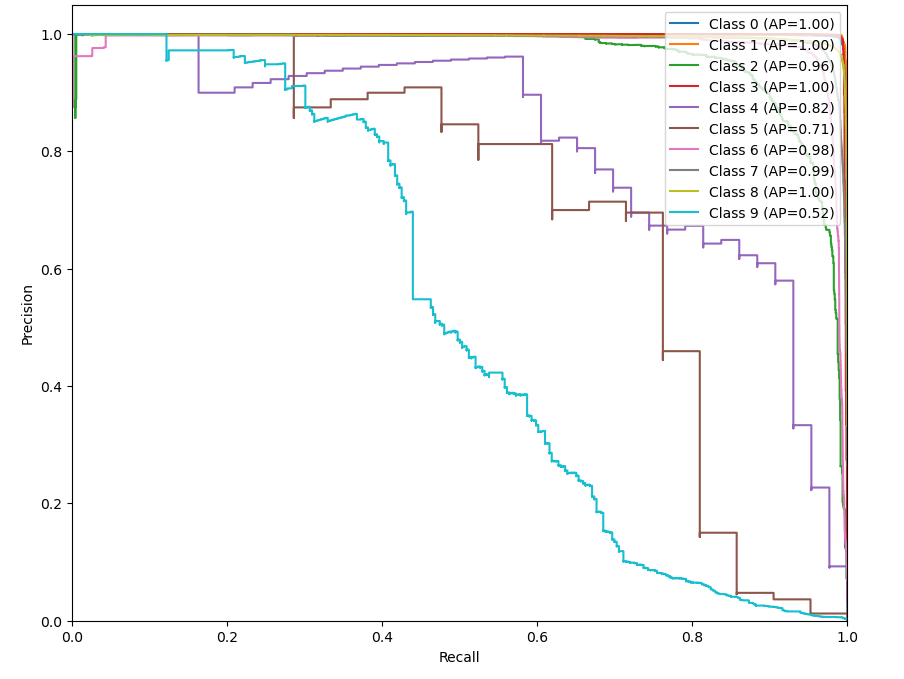
\includegraphics[width=0.6\textwidth]{pr_good.png}
\end{figure}

Наблюдаем хорошие показатели классификации для префикса длины 3.
\end{frame}

%%%%%%%%%%%%%%%%%%%%%%%%%%%%%%%%%%%%%%
\begin{frame}{Вычислительный эксперимент}
\scriptsize % Уменьшает размер шрифта для содержимого таблицы

\begin{table}[htb]
\centering
\begin{tabular}{|l|l|l|l|l|l|l|l|}
\hline
\textbf{Text}  & \textbf{1 st} & \textbf{1.5 st} & \textbf{2 st} & \textbf{2.5 st} & \textbf{3 st} & \textbf{4 st} & \textbf{Embedding} \\ \hline
укроп свежий  & 1 & 11 & 113 & 1131 & 11319 & 11319000 & [0.3,0.2..] \\ \hline
яблоки  & 1 & 12 & 124 & 1241 & 12410 & 12410000 & [-0.2,0.3..] \\ \hline
\end{tabular}
\end{table}

\vspace{1em} % Добавляет вертикальное пространство

\begin{figure}[htb]
\centering
\includegraphics[width=1\textwidth]{new_pr.png}
\end{figure}

\end{frame}

%----------------------------------------------------------------------------------------------------------
\begin{frame}{Иерархическая классификация}
 Мы достаточно хорошо умеем прогнозировать префиксы 3-4, а так как данные имеют иерархическую структуру, хотелось бы использовать результаты предсказания первых цифр при предсказании дальнейших.
\begin{itemize}
    \item Эксперимент 1: Будем добавлять предсказанные цифры в вектор признаков. 
    \item Эксперимент 2: Будем разделять выборку на подклассы, по результатам классификации по первым цифрам. Далее для каждого класса - обучаем свою модель. 
    
\end{itemize}
Идеи похожи друг на друга. Вторая по сути представляет собой более строгое использование результата предыдущей классификации, по сравнению с первой.
\end{frame}
%----------------------------------------------------------------------------------------------------------

%----------------------------------------------------------------------------------------------------------
\begin{frame}{Сравнение способов}

Выборка одна и та же, всего 736 тысяч записей.\\
Так как всё же эксперименты чуть отличаются --- не можем сравнивать их графики roc и pr. Будем анализировать качество модели, в зависимости от ступени: \\
\bigskip \\

\begin{tabular}{|l|c|c|c|}

\hline

\textbf{Method} & \textbf{Standart} & \textbf{Class split} & \textbf{Hierarchical} \\ \hline
prefix 4 & 87.6\% & 88.4\% & 88.2\% \\ \hline
prefix 5 & 85.6\% & 86.4\% & 86.1\% \\ \hline
prefix 6 & 83.7\% & 84.9\% & 84.7\% \\ \hline
\end{tabular}

\bigskip  \\
В таблице представлено количество правльных ответов модели (в процентах) в зависимости от метода. Standart - обычный способ, Class split - с разделением на классы, Hierarchical --- с добавлением нового признака.\\
\textbf{Вывод:} Относительное количество ошибок уменьшилось примерно на 5\%, абсолютная точность эксперимента - на 1\%. При этом время и вычислительная сложность увеличились в разы.

\end{frame}
%----------------------------------------------------------------------------------------------------------
\begin{frame}{Заключение}
    
    \begin{itemize}
        \item Предложен алгоритм для решения поставленной задачи классификации.
        \item Реализована модель выполняющая этот алгоритм
        \item Исследовано влияние гиперпараметров на результаты модели 
        \item Исследовано качество модели в зависимости от глубины классификатора
        \item Исследованы методы улучшенния модели и их качество
    \end{itemize}

    Пути улучшения:
    \begin{itemize}
        \item Улучшение качества эмбеддингов
        \item Объединение и усовершенствование предложенных улучшенных методов классификации
        \item Борьба с несбалансированностью классов
    \end{itemize}
    
\end{frame}
%----------------------------------------------------------------------------------------------------------
%----------------------------------------------------------------------------------------------------------
\begin{frame}{Список литературы}
\begin{itemize}
    \item Lane, H., Howard, C., \& Hapke, H. (2019). \textit{Natural Language Processing in Action}. Manning Publications. 
    \item Marra de Artiñano, I., Riottini Depetris, F., \& Volpe Martincus, C. (2021). \textit{Automatic Product Classification in International Trade: Machine Learning and Large Language Models}. 
    \item Lewis, D. D., et al. (2004). \textit{RCV1: A New Benchmark Collection for Text Categorization Research.} Journal of Machine Learning Research, 5. 
    \item Haav, H.-M. (2021). \textit{Assessment of HS Code Correctness}. 
    \item Muñoz, E. (2020). \textit{Introduction to Natural Language Processing: Word Embeddings \& Sentiment Analysis with Python}. 
    %\item Montani, I. (2019). \textit{Advanced NLP with spaCy: A Practical Guide to Advanced Natural Language Processing}. Independent.
\end{itemize}
\end{frame}

%----------------------------------------------------------------------------------------------------------

\end{document} 
